An alternative \dword{adc} solution is to adapt the \dword{adc} chip under development for the 
ATLAS \lar calorimeter readout upgrade for the HL-LHC.  The main ATLAS 
requirements are given in Table~\ref{tab:ATLAS-adc-reqs}.  Adapting the chip to %DUNE 
the \dword{spmod} needs 
would require doubling the number of channels per chip as well as adapting the output 
architecture.  These are both relatively simple changes compared to the overall complexity of the chip.

\begin{dunetable}
[Performance requirements for the ATLAS-style \dword{adc} \dword{asic}.]
{ll}
{tab:ATLAS-adc-reqs}
{Performance requirements for the ATLAS-style \dword{adc} \dword{asic}.}
\textbf{Parameter} &\textbf{Specification}\\ \toprowrule
Channels/chip & eight preferred, four minimum \\ \colhline
Sampling Frequency & \SI{40}{MHz} \\ \colhline
Dynamic Range & \SI{14}{bits}  \\ \colhline
Precision & \SI{11}{ENOB}\\ \colhline
Power & $<$~\SI{100}{mW}/channel at \SI{40}{MHz}\\ \colhline
Input & \SI{2}{V} differential\\ \colhline
Output & E-link interface operating at \SI{640}{Mbps}\\
\end{dunetable}

To achieve a \SI{14}{bit} dynamic range, each analog channel is comprised
of two main sections: a Dynamic Range Enhancement (\dword{dre}) block that determines the
most significant two bits of the \SI{14}{bit} digital code, followed by a \SI{12}{bit} \dword{sar} block. %The design of the \dword{dre} is shown schematically in Figure~\ref{fig:65nm\dword{adc}architecture_dre}.
The input signal to the \dword{dre} block is sampled on two
paths, one with unity gain and the other of gain four. A comparator determines which gain to use.
The signal from the selected \dword{dre} gain is presented at the \dword{dre} output,
which is connected to the input of the \SI{12}{bit} \dword{sar} \dword{adc} block. The \dword{dre} design has been carefully
optimized so that its output preserves the required \SI{12}{bit} performance.

%\begin{dunefigure}
%[Block diagram of the \dword{dre} architecture for the ATLAS \dword{adc} \dword{asic}.]
%{fig:65nm\dword{adc}architecture_dre}
%{Block diagram of the \dword{dre} architecture for the ATLAS \dword{adc} \dword{asic}.}
%\includegraphics[width=.55\textwidth]{tpcelec-\dword{dre}concept_resized.pdf}
%\end{dunefigure}

Following current state-of-the-art \dword{adc} development techniques, a two-stage 
\dword{sar} architecture is used, exploiting the high speed of the technology while maintaining the \dword{sar} input 
capacitance at a reasonable value. Since capacitor matching in this technology might not meet the 
precision required, the \dword{adc} will use bit redundancy, i.e., determine more bits than its actual output, 
and the redundant bits will be used to both calibrate the \dword{adc} and produce correct output codes. 
Such procedures are well understood and applied to both pipeline~\cite{Kuppambatti:2013nfa} and 
\dword{sar}~\cite{5999734} \dwords{adc} using foreground or background calibration techniques. Details of the \dword{sar} design are shown in Figure~\ref{fig:65nmadcarchitecture_sar}. 

\begin{dunefigure}
[Block diagram of the two-stage \dword{sar} design of the ATLAS \dword{adc} \dword{asic}.]
{fig:65nmadcarchitecture_sar}
{Block diagram depicting the two-stage \dword{sar} design of the ATLAS \dword{adc} \dword{asic}.}
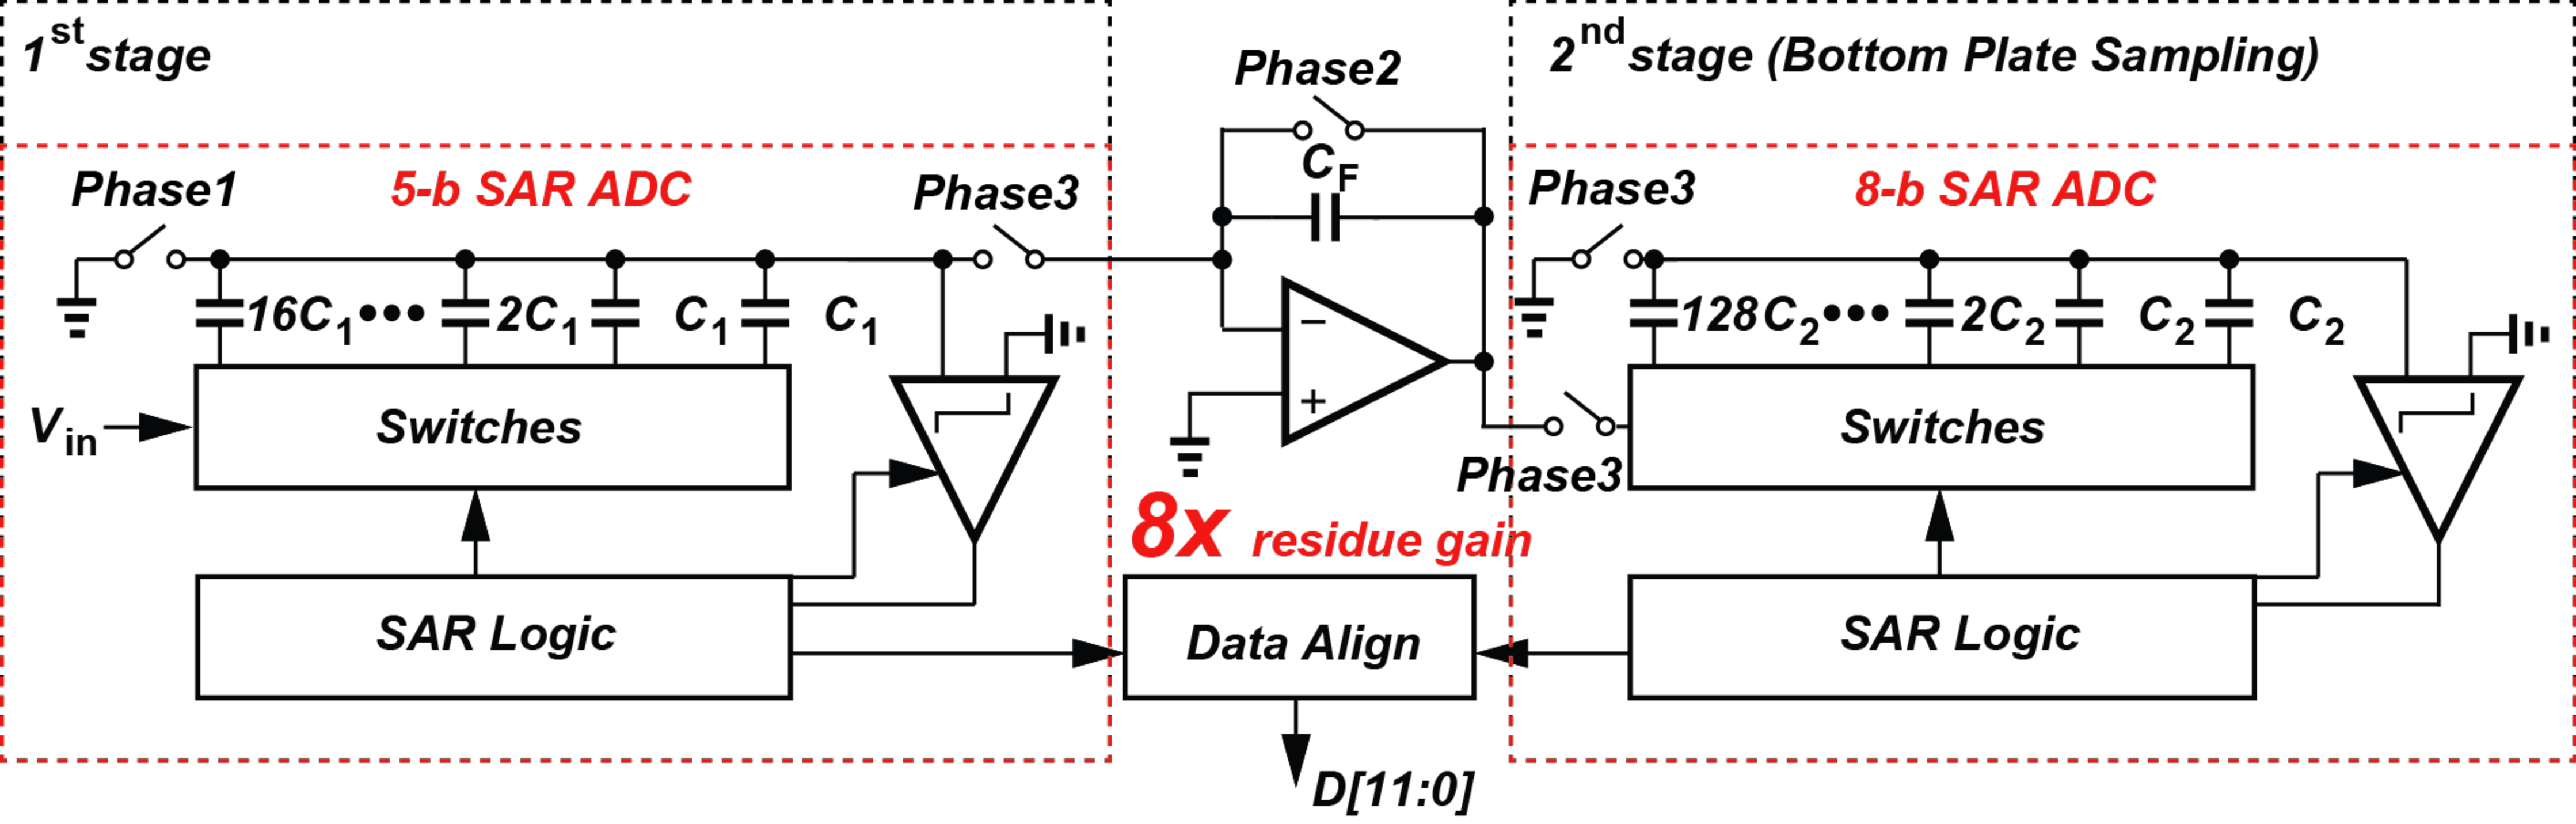
\includegraphics[width=.9\textwidth]{tpcelec-SARdesign.pdf}
\end{dunefigure}

An \dword{adc} test chip, dubbed \textit{COLUTA65V1}, was designed and submitted for fabrication in May 2017 and received
in September of 2017.  The \dword{dre} and \dword{sar} blocks of the COLUTA65V1 were first tested independently. Measurements were made of the \dword{sar} precision using the sine-wave Fast Fourier Transform method. An effective number of bits
(ENOB) of \SI{11.6}{bits} at \SI{20}{MHz} (after calibration) was obtained.
%Similar measurements at \SI{40}{MHz} do not match the expected performance and 
%additional testing and simulation indicates that the layout of the connection between the first \dword{sar} stage and the amplifier is not optimal. Similar results were observed with
%the \dword{dre} performance and again simulation indications improvements are possible in the layout. 
%The next submission of the chip, planned for Spring 2018, will incorporate this work in the iteration 
%of the design.
Both \dword{dre} and \dword{sar} were successfully integrated with negligible degradation in performance. The COLUTA65V1 chip was also tested at \SI{2}{MHz} and shown to work as designed, meeting the requirement for the \dword{spmod}. % DUNE. 
Tests of an updated design in liquid nitrogen are planned for spring 2018. Additional tests associated with meeting power requirements will be carried out if this \dword{adc} option is further pursued.
